%%
%% (
%%  )\ )                             (
%%  (()/(   (            (             )\  )   (
%%   /(_))  ))\   (       ))\  (   (   (()/(   ))\
%%   (_))  /((_)  )\  )  /((_) )\  )\   ((_))/((_)
%%   | _ \(_))(  _(_/( (_) )  ((_)((_)  _| |(_))
%%   |   /| || || ' \))/ -_)/ _|/ _ \/ _` |/ -_)
%%   |_|_\ \_,_||_||_| \___|\__|\___/\__,_|\___|
%%

\documentclass{article}
\usepackage[utf8x]{inputenc}
\usepackage{amsmath}
%\usepackage{slashbox}
\usepackage{amsfonts}
\usepackage{amssymb}
\usepackage{graphicx} % Paquete para incluir imágenes en el documento LaTeX
\usepackage{hyperref}
\hypersetup{
  colorlinks=true,
  linkcolor=blue,
  filecolor=magenta,
  urlcolor=cyan,
}
\urlstyle{same}
\usepackage{varwidth}

\newcommand\tab[1][1cm]{\hspace*{#1}}

\usepackage{multirow}

\usepackage[a4paper,rmargin=1.5cm,lmargin=1.5cm,top=1.5cm,bottom=1.5cm]{geometry}

\usepackage{pdfpages}

\usepackage{xcolor}
\usepackage{minted}
\usemintedstyle[cpp]{monokai}
\usemintedstyle[python]{paraiso-dark}
\usemintedstyle[./pseudocode.py:PseudocodeLexer -x]{rainbow_dash}
\definecolor{LightGray}{gray}{0.98}
\definecolor{DarkGray}{gray}{0.1}
\definecolor{MidGray}{gray}{0.8}
\definecolor{codegreen}{rgb}{0,0.6,0}
\definecolor{codegray}{rgb}{0.5,0.5,0.5}
\definecolor{codepurple}{rgb}{0.58,0,0.82}
\definecolor{backcolour}{rgb}{0.95,0.95,0.92}

\setlength{\parindent}{0px}  % Setea la indentacion de la primera linea de cada parrafo a cero pixeles.


\title{Resolución de la primera semana}
\author{@RuneCode}

\begin{document}
%% Portada
\includepdf{./portada/portada.pdf}


%% ####################################################################################
%%    Inicio del Documento
%% ####################################################################################
\section*{Quinta Semana}%
En esta clase se revisaron los temas de:
\begin{itemize}
\item \textbf{Programación modular}
\item \textbf{Subprogramas}
\item \textbf{Procedimiento}
\item \textbf{Declaración, Definición y Llamada}
\item \textbf{Función}
\item \textbf{Ámbito de variables local y global}
\item \textbf{Paso de parámetros por valor y referencia}
\end{itemize}
\vspace{1cm}
\textbf{Nota:} Te recomendamos realizar los ejercicios antes de ver su solución
ya que el objetivo de este documento es presentarte una de las muchas posibles
soluciones y así tengas una modelo con el que puedas comparar. Si tienes alguna
sugerencia de mejora puedes comunicarte por correo a la dirección
\href{mailto:gprunecode@gmail.com}{gprunecode@gmail.com}.

\section{Programación Modular}%
La programación modular es una metodología de programación que consiste en organizar un programa en módulos.\\
En la etapa de diseño de un programa se aplica la \textbf{estrategia "divide y vencerás".}\\
En la \underline{etapa de implementación}, cada uno de los subproblemas se implementa a través de un módulo.\\
Los lenguajes de programación brindan diferentes mecanismos para implementar módulos.
Los módulos más simples son los procedimientos y funciones.\\

\section{Subprogramas}%
\textbf{Subprogramas:} bloques de código que llevan a cabo una tarea concreta (resuelven un subproblema concreto)
\begin{itemize}
  \item Tienen un propósito
  \item Tienen unas precondiciones
  \item Permiten reutilizar código de manera sencilla y segura. Pueden ser usados más de una vez en el programa
        principal sin necesidad de reescribir todo (o copiar-pegar).
  \item Ayudan a que el código del programa principal sea: \textbf{legible:} resulta más sencillo leer sólo el
        nombre del subprograma que todo su código, \textbf{ordenado:} cada subprograma ocupa un lugar concreto
        dentro de todo el código.
\end{itemize}

\subsection*{Ejemplo 1}%
Hallar el cociente y resto de una división.\\

%Pseudocódigo
\underline{\textit{Resolución en pseudocódigo}}\\ 
\inputminted
[
  frame=lines,
  framesep=2mm,
  baselinestretch=1.2,
  rulecolor=\color{black!30},
  %fontsize=\footnotesize,
  bgcolor=LightGray,
  %linenos
]
{./pseudocode.py:PseudocodeLexer -x}
{./pseudocodigo/001_ejemplo.algo}

%C++
\underline{\textit{Resolución en C++}}\\
\inputminted
[
  frame=lines,
  framesep=2mm,
  baselinestretch=1.2,
  rulecolor=\color{black!30},
  %fontsize=\footnotesize,
  bgcolor=DarkGray,
  %linenos
]
{cpp}
{./cpp/001_ejemplo.cpp}


\section{Procedimiento}%
Son \textbf{subprogramas} que realizan una tarea determinadad y devuelven 0 o
más de un valor. Se utilizan para estructurar un programa y mejorar su claridad
y generalidad.\\
Debido a que devuelven más de un resultado, \textbf{NO UTILIZAN} la palabra
reservada \textbf{retornar} y los parámetros pueden ser:
\begin{itemize}
  \item \textbf{de ENTRADA} Sólo se utilizan para que los subprogramas que llaman al procedimiento le pasen datos al
        mismo.
  \item \textbf{de ENTRADA/SALIDA} Se utilizan por parte de los subprogramas que llaman, para pasarle datos al
        procedimiento para pasar los resultados obtenidos al subprograma que lo ha llamado.
\end{itemize}

\subsection{Procedimiento: Declaración, Definición, Llamada}%

%Pseudocódigo
\inputminted
[
  frame=lines,
  framesep=2mm,
  baselinestretch=1.2,
  rulecolor=\color{black!30},
  %fontsize=\footnotesize,
  bgcolor=LightGray,
  %linenos
]
{./pseudocode.py:PseudocodeLexer -x}
{./pseudocodigo/procedimiento.algo}

\subsection*{Ejemplo 2}%

%Pseudocódigo
\underline{\textit{Resolución en pseudocódigo}}\\ 
\inputminted
[
  frame=lines,
  framesep=2mm,
  baselinestretch=1.2,
  rulecolor=\color{black!30},
  %fontsize=\footnotesize,
  bgcolor=LightGray,
  %linenos
]
{./pseudocode.py:PseudocodeLexer -x}
{./pseudocodigo/002_ejemplo.algo}

%C++
\underline{\textit{Resolución en C++}}\\
\inputminted
[
  frame=lines,
  framesep=2mm,
  baselinestretch=1.2,
  rulecolor=\color{black!30},
  %fontsize=\footnotesize,
  bgcolor=DarkGray,
  %linenos
]
{cpp}
{./cpp/002_ejemplo.cpp}


\section{Función}%
Son subprogramas que realizan una determinada tarea y devuelven un único resultado o valor. Se utilizan para crear
operaciones nuevas no incluidas en el lenguaje.\\
El resultado devuelto se indica mediante la palabra reservada \textbf{retornar}, y \textbf{TODOS LOS PARÁMETROS} son
de \textbf{ENTRADA}.

%Pseudocódigo
\inputminted
[
  frame=lines,
  framesep=2mm,
  baselinestretch=1.2,
  rulecolor=\color{black!30},
  %fontsize=\footnotesize,
  bgcolor=LightGray,
  %linenos
]
{./pseudocode.py:PseudocodeLexer -x}
{./pseudocodigo/funcion.algo}

\subsection*{Ejemplo 3}%
Escribir subprograma para hallar el factorial de un número.\\

%Pseudocódigo
\underline{\textit{Resolución en pseudocódigo}}\\ 
\inputminted
[
  frame=lines, framesep=2mm,
  baselinestretch=1.2,
  rulecolor=\color{black!30},
  %fontsize=\footnotesize,
  bgcolor=LightGray,
  %linenos
]
{./pseudocode.py:PseudocodeLexer -x}
{./pseudocodigo/003_ejemplo.algo}

%C++
\underline{\textit{Resolución en C++}}\\
\inputminted
[
  frame=lines,
  framesep=2mm,
  baselinestretch=1.2,
  rulecolor=\color{black!30},
  %fontsize=\footnotesize,
  bgcolor=DarkGray,
  %linenos
]
{cpp}
{./cpp/003_ejemplo.cpp}

Como vemos, no está presente la función \textbf{principal} llamada \textbf{main} en C++, en el archivo fuente
llamado \textbf{003\_ejemplo.cpp}. Podemos llamar el codigo de este fichero fuente desde otro de la siguiente
manera:

%C++
\inputminted
[
  frame=lines,
  framesep=2mm,
  baselinestretch=1.2,
  rulecolor=\color{black!30},
  %fontsize=\footnotesize,
  bgcolor=DarkGray,
  %linenos
]
{cpp}
{./cpp/prueba.cpp}



\section{Ámbito de variables}%
El buen uso de la programación modular requiere que los módulos sean independientes.\\
Esto se consigue intentando satisfacer dos condiciones:
\begin{itemize}
  \item Cada módulo se diseña sin conocimiento del diseño de otros módulos.
  \item La ejecución de un subprograma particular no tiene por que afectar a los valores de las variables de otros
        subprogramas.
\end{itemize}
Dado que se permite el anidamiento en la llamada a subprogramas, es necesario evitar problemas con los
identificadores definidos en varias partes del código.\\

\subsection*{Ejemplo}%
%Pseudocódigo
\underline{\textit{Resolución en pseudocódigo}}\\ 
\inputminted
[
  frame=lines,
  framesep=2mm,
  baselinestretch=1.2,
  rulecolor=\color{black!30},
  %fontsize=\footnotesize,
  bgcolor=LightGray,
  %linenos
]
{./pseudocode.py:PseudocodeLexer -x}
{./pseudocodigo/004_ejemplo.algo}

%C++
\underline{\textit{Resolución en C++}}\\
\inputminted
[
  frame=lines,
  framesep=2mm,
  baselinestretch=1.2,
  rulecolor=\color{black!30},
  %fontsize=\footnotesize,
  bgcolor=DarkGray,
  %linenos
]
{cpp}
{./cpp/cuadratica.cpp}


\subsection{Ámbito de variables: Variable Local}%
Son aquellas que se declaran en el cuerpo de la función. Solo son "visibles" o "usables" dentro de la función
donde se han declarado.\\
Dos funciones diferentes, pueden utilizar los mismos nombres de variables sin "interferencias" ya que se
refieren a posiciones diferentes de memoria.\\

\begin{figure}[h!]
  \centering
  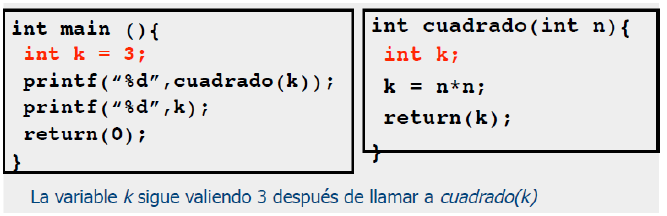
\includegraphics[scale=0.75]{./pictures/variables_locales.png}
\end{figure}

%Pseudocódigo
\underline{\textit{Resolución en pseudocódigo}}\\ 
\inputminted
[
  frame=lines,
  framesep=2mm,
  baselinestretch=1.2,
  rulecolor=\color{black!30},
  %fontsize=\footnotesize,
  bgcolor=LightGray,
  %linenos
]
{./pseudocode.py:PseudocodeLexer -x}
{./pseudocodigo/variableLocal.algo}

%C++
\underline{\textit{Resolución en C++}}\\
\inputminted
[
  frame=lines,
  framesep=2mm,
  baselinestretch=1.2,
  rulecolor=\color{black!30},
  %fontsize=\footnotesize,
  bgcolor=DarkGray,
  %linenos
]
{cpp}
{./cpp/potenciaCuadrado.cpp}


\subsection{Ámbito de variables: Variable Global}%
Es aquella que se define fuera del cuerpo de cualquier función, normalmente al principio del programa y antes de
cualquier función (En C++ después de la definición de los archivos de biblioteca (\#include) y de la definición de
constantes simbólicas).\\
El ámbito de una variable global son todas las funciones que componen el programa, cualquier función puede acceder a
dichas variables para leer y escribir en ellas. Es decir, se puede hacer referencia a su dirección de memoria en
cualquier parte del programa.\\
Al programar usando procedimientos y funciones, no utilizaremos en nuestras apliaciones las variables globales, pues
atenta contra la modularidad y el bajo acoplamiento que son lo que deseamos.\\

%C++
\inputminted
[
  frame=lines,
  framesep=2mm,
  baselinestretch=1.2,
  rulecolor=\color{black!30},
  %fontsize=\footnotesize,
  bgcolor=DarkGray,
  %linenos
]
{cpp}
{./cpp/variableGlobal.cpp}

\section{Parámetros actuales o reales}%
Son las variables de enlace definidas en el programa principal y que se usan como argumentos dentro de los paréntesis
que posee una llamada a un subprograma.

%Pseudocódigo
\underline{\textit{Resolución en pseudocódigo}}\\ 
\inputminted
[
  frame=lines,
  framesep=2mm,
  baselinestretch=1.2,
  rulecolor=\color{black!30},
  %fontsize=\footnotesize,
  bgcolor=LightGray,
  %linenos
]
{./pseudocode.py:PseudocodeLexer -x}
{./pseudocodigo/actualesReales.algo}

\begin{figure}[h!]
  \centering
  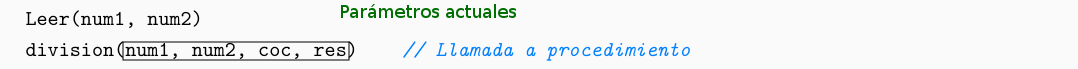
\includegraphics[scale=0.63]{./pictures/parametros_actuales.png}
\end{figure}

\section{Parámetros formales o ficticios}%
Son las variables de enlace definidas en la entrada de un subprograma que aceptan los valores de los parámetros
actuales que se usan en la llamada al subprograma y se comportan como otras variables locales.\\

%Pseudocódigo
\inputminted
[
  frame=lines,
  framesep=2mm,
  baselinestretch=1.2,
  rulecolor=\color{black!30},
  %fontsize=\footnotesize,
  bgcolor=LightGray,
  %linenos
]
{./pseudocode.py:PseudocodeLexer -x}
{./pseudocodigo/parametroFormal.algo}

\begin{figure}[h!]
  \centering
  
\includegraphics[scale=0.63]{./pictures/parametros_formales.png}
\end{figure}

\section{Paso de parámetros: Por valor}%
El paso de parámetros por valor consiste en copiar el contenido de la variable que queremos pasar en otra dentro del
ámbito local del subprograma. Se tendrán dos valores duplicados e independientes, con lo que la modificación de uno
no afecta al otro.
\newpage

\begin{figure}[h!]
  \centering
  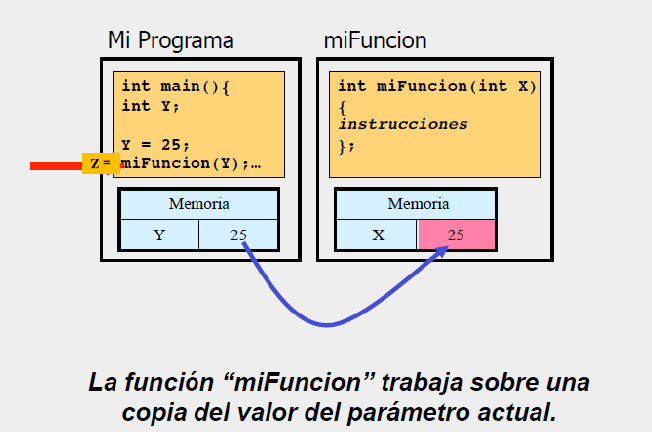
\includegraphics[scale=0.75]{./pictures/paso_por_valor.png}
\end{figure}

%Pseudocódigo
\underline{\textit{Resolución en pseudocódigo}}\\ 
\inputminted
[
  frame=lines,
  framesep=2mm,
  baselinestretch=1.2,
  rulecolor=\color{black!30},
  %fontsize=\footnotesize,
  bgcolor=LightGray,
  %linenos
]
{./pseudocode.py:PseudocodeLexer -x}
{./pseudocodigo/pasoPorValor.algo}

%C++
\underline{\textit{Resolución en C++}}\\
\inputminted
[
  frame=lines,
  framesep=2mm,
  baselinestretch=1.2,
  rulecolor=\color{black!30},
  %fontsize=\footnotesize,
  bgcolor=DarkGray,
  %linenos
]
{cpp}
{./cpp/potenciaCuadrado.cpp}


\section{Paso por parámetros: Por referencia}%
El paso de parámetros por referencia consiste en proporcionar al subprograma al que se quiere pasar el argumento,
la \textbf{dirección de memoria} del dato. En este caso se tiene un único valor referenciado (o apuntado) desde dos
puntos diferentes, el programa principal y subprograma al que se pasa el argumento por lo que cualquier acción sobre
el parámetro se realiza sobre el mismo dato en la memoria.\\

\begin{figure}[h!]
  \centering
  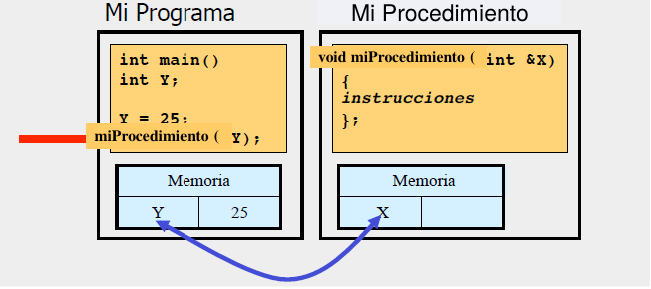
\includegraphics[scale=0.75]{./pictures/paso_por_referencia.png}
\end{figure}

La variable \textbf{X} es en realidad una dirección de memoria que apunta a la variable \textbf{Y}. Para poder usar
\textbf{X} tendremos que anteponer siempre un \textbf{\&}.\\
Todos los cambios que hagamos dentro del procedimiento \textit{"miProcedimiento"} sobre la variable \textbf{X} se
reflejarán en el parámetro actual correspondiente, en este caso \textbf{Y}.\\

%Pseudocódigo
\inputminted
[
  frame=lines,
  framesep=2mm,
  baselinestretch=1.2,
  rulecolor=\color{black!30},
  %fontsize=\footnotesize,
  bgcolor=LightGray,
  %linenos
]
{./pseudocode.py:PseudocodeLexer -x}
{./pseudocodigo/pasoPorReferencia.algo}

\subsection*{Ejercicio 1}%
Use subprogramas y paso de parámetros para hallar la suma de los n términos de:
\begin{equation*}
  1 + \frac{1}{2!} + \frac{1}{3!} + \frac{1}{4!} + \cdots
\end{equation*}

%Pseudocódigo
\underline{\textit{Resolución en pseudocódigo}}\\ 
\inputminted
[
  frame=lines,
  framesep=2mm,
  baselinestretch=1.2,
  rulecolor=\color{black!30},
  %fontsize=\footnotesize,
  bgcolor=LightGray,
  %linenos
]
{./pseudocode.py:PseudocodeLexer -x}
{./pseudocodigo/001_ejercicio.algo}

%C++
\underline{\textit{Resolución en C++}}\\
\inputminted
[
  frame=lines,
  framesep=2mm,
  baselinestretch=1.2,
  rulecolor=\color{black!30},
  %fontsize=\footnotesize,
  bgcolor=DarkGray,
  %linenos
]
{cpp}
{./cpp/001_ejercicio.cpp}


\subsection*{Ejercicio 2}%
Usando subprogramas halle las raíces de la ecuación cuadrática.\\

%Pseudocódigo
\underline{\textit{Resolución en pseudocódigo}}\\ 
\inputminted
[
  frame=lines,
  framesep=2mm,
  baselinestretch=1.2,
  rulecolor=\color{black!30},
  %fontsize=\footnotesize,
  bgcolor=LightGray,
  %linenos
]
{./pseudocode.py:PseudocodeLexer -x}
{./pseudocodigo/002_raicesCuadratica.algo}


%C++
\underline{\textit{Resolución en C++}}\\
\inputminted
[
  frame=lines,
  framesep=2mm,
  baselinestretch=1.2,
  rulecolor=\color{black!30},
  %fontsize=\footnotesize,
  bgcolor=DarkGray,
  %linenos
]
{cpp}
{./cpp/002_ejercicio.cpp}

\section*{Agradecimientos}
\textbf{Personas que apoyaron mandando psudocódigo y código en este documento:}\\

%---------------------------------------------------------------------------------
\vspace{3cm} 
\section*{¡Envianos tus soluciones!}
Si estás llevando este curso con los profesores Cabrera, Romero o Salinas;
envíanos tus soluciones en los diferentes lenguajes de programación que
conozcas al correo \href{mailto:gprunecode@gmail.com}{gprunecode@gmail.com}.
n.n \\ 

Las mejores soluciones tanto en el algoritmo como en el código, serán
publicadas en las siguientes ediciones de estos documentos.\\ \\

El asunto del correo debe estar de la siguiente manera:\\
$NumeroDeSesion-Profesor-NumeroDeEjercicio$ \\ \\
Por ejemplo:  \\
$01-Romero-01$ \\

Y dentro del correo adjuntar tu solución y nombre como quieras ser reconocido en caso de ser electo.

\vspace{2cm}
\LARGE\textit{RuneCode}


\end{document}

